\chapter{基于状态模型的信号估计}
\label{chap:state-space-estimation}

传感器读数是我们能拿到的信号，产生读数的系统内部却有一个看不见的状态：房间的真实温度、目标的真实位置。
如果知道状态怎样一步步演化、传感器又怎样把状态变成带噪读数，就能反过来问：读到这串信号以后，状态最可能在哪里？
本章在给定状态模型的前提下回答这个问题，依次研究推断目标、预测、滤波、平滑与整条轨迹的推断。

状态模型的生成部分沿用\BookChapterRef{chap:discrete-time-stochastic-processes}{“离散时间随机过程”章}的转移核语言：
初态服从$\pi_0$，给定当前状态$\bm x_t$与已知输入$\bm u_t$后，下一状态由概率核$K_t(\bm x_t,\cdot)$生成，且与更早的历史条件独立。
最常用的是线性加性模型
\begin{equation}
  \bm x_{t+1}=\bm A_t\bm x_t+\bm B_t\bm u_t+\bm w_{t+1},
  \label{eq:dynamical-linear-state-model}
\end{equation}
其中过程噪声$\bm w_{t+1}\sim\mathcal N(\bm0,\bm Q_{t+1})$独立于初态和其他时刻的噪声，于是$K_t(\bm x,\cdot)=\mathcal N(\bm A_t\bm x+\bm B_t\bm u_t,\bm Q_{t+1})$。
贯穿全章的温度例取标量$x_{t+1}=0.8x_t+u_t+w_{t+1}$，$w_{t+1}\sim\mathcal N(0,0.04)$，初态$x_0=0$，输入恒为$u_t=0.4$；
此时$\mathbb E x_t=2(1-0.8^t)$，一条实际轨迹在平均轨迹附近波动。
图~\ref{fig:action-state-temperature-layers}再叠加独立读数噪声$v_t\sim\mathcal N(0,0.09)$，得到读数$y_t=x_t+v_t$，展示演化规律、真实状态与读数三个层次。

\begin{figure*}[htbp]
  \centering
  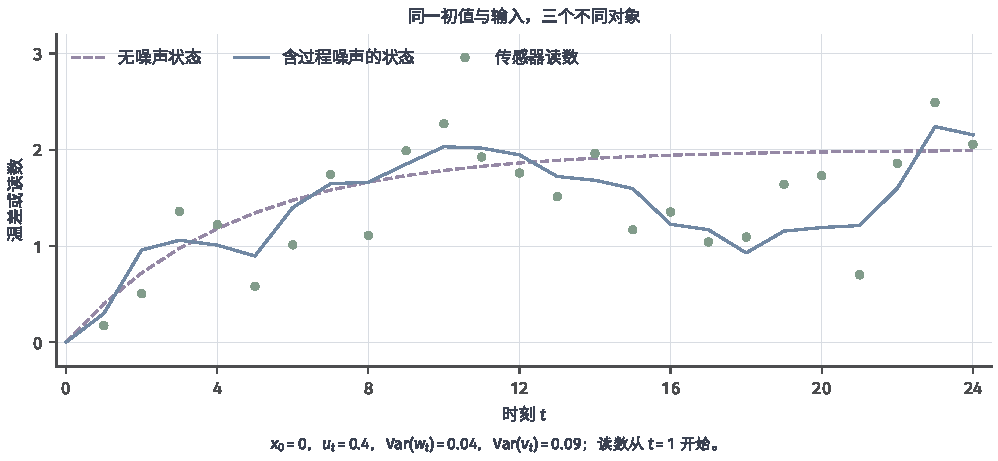
\includegraphics[width=\linewidth]{figures/00-shared/mathematical-preliminaries-lower/02-dynamical-systems-control-decision-and-games/matplotlib/action-state-temperature-layers/figure.pdf}
  \caption{同一温度模型的三个对象。初态$x_0=0$，输入始终为$0.4$；
  无噪声轨迹趋于$2$，过程噪声改变真实状态，独立观测噪声又把真实状态变成带噪读数。
  噪声方差分别为$0.04$和$0.09$。图中带噪曲线是固定种子的教学模拟，
  不是置信区间，也没有把读数用于反向校正状态。}
  \label{fig:action-state-temperature-layers}
\end{figure*}

过程噪声规定真实状态如何随机移动；但真实状态往往无法直接读取，只能通过带误差的传感器间接观测——温度计有读数误差、雷达只能测距离而测不到完整位置。于是出现一个反向问题：给定一串传感器读数，怎样反推产生它们的隐藏状态轨迹？
因此推断不是再次生成一条任意轨迹，而是在已给定的生成模型中，保留与读数相容的
状态并重新分配概率：读数支持哪些状态，就提高它们的可能性，排除与之矛盾的状态。先明确已取得的传感器读数与所求状态量，再把预测、滤波和平滑化为可计算公式。

\section{观测条件下的推断目标}
在前面的状态转移$K_t$之外增加观测核
$G_t(\bm x,B)=\mathbb P(\bm y_t\in B\mid\bm x_t=\bm x)$。
它表示状态为$\bm x$时传感器返回哪些读数。线性加性例为
\begin{equation}
  \bm y_t=\bm C_t\bm x_t+\bm v_t.
  \label{eq:dynamical-linear-observation-model}
\end{equation}
先假设初值、所有过程噪声与所有观测噪声相互独立，输入与矩阵给定。
于是给定$\bm x_t$后，$\bm y_t$不再依赖旧状态和旧观测；
给定当前状态后，下一状态由$K_t$生成。联合规律在
式~\eqref{eq:dynamical-linear-state-model}的基础上分解为
\[
 \pi_0(\mathrm d\bm x_0)
       \prod_{t=0}^{T-1}K_t(\bm x_t,\mathrm d\bm x_{t+1})
       \prod_{t=1}^T G_t(\bm x_t,\mathrm d\bm y_t).
\]
这里从$y_1$开始观察，$\pi_0$不含一个未声明的$y_0$。
若噪声相关、传感器依赖旧状态或有内部滞后，须扩充联合状态或显式改写这些
条件关系。观测序列通常不满足自身的Markov性，因为一次带噪读数未必概括隐藏状态。

记$\mathcal Y_t=\sigma(\bm y_1,\ldots,\bm y_t)$，
$\mathcal Y_0$为无观测信息。欧氏状态与观测具有正则条件分布，
使“给定这段读数的状态概率”能作为概率核处理。
即使观测无噪，也不一定足够：$y_t=x_{1,t}+x_{2,t}$不能区分
$(1,0)^\top$与$(0,1)^\top$。能否借后续动力学区分这些方向，需要
\BookChapterRef{chap:control-theory}{第~\ref{chap:control-theory}章}的可观测性与可检测性条件。

这里“借后续动力学区分”可以算一遍。在一个无噪教学例中，设时刻$1$的状态
$\bm x_1$有$(1,0)^\top$或$(0,1)^\top$两个候选。
读数$y_1=x_{1,1}+x_{2,1}$对它们都等于$1$，仅凭它无法判断分量如何分配。
若动力学为$\bm x_{t+1}=\bm A\bm x_t+\bm u_t$，其中
$\bm A=\operatorname{diag}(0.5,2)$，在读得$y_1$之后施加共同已知输入
$\bm u_1=(0.5,0)^\top$，则时刻$2$的两个候选分别为
\[
 \bm A(1,0)^\top+\bm u_1=(1,0)^\top,\qquad
 \bm A(0,1)^\top+\bm u_1=(0.5,2)^\top.
\]
因此下一次读数$y_2=x_{1,2}+x_{2,2}$分别为$1$与$2.5$，两者便被分开。
共同输入在两个候选的状态差中相互抵消；区别来自状态转移把原先看不到的分量差
带入下一次读数。这个例子说明可观测性要连同状态转移
一起判断：一次观测丢掉的信息，可能被后续演化重新带到观测方向，也可能始终留在
看不到的子空间里。

\begin{example}[带泄漏温度的间接观测]
 \label{ex:dynamical-noisy-temperature}
 回到同一模型
 $x_{t+1}=0.8x_t+u_t+w_{t+1}$、$y_t=x_t+v_t$，
 其中$w_t\sim\mathcal N(0,0.04)$、$v_t\sim\mathcal N(0,0.09)$，
 与初值及彼此独立。即使传感器完全精确，未来仍因$w_{t+1}$不确定；
 即使过程无噪，当前状态也可能因读数噪声而不确定。
 图~\ref{fig:action-state-temperature-layers}的轨迹从已知$x_0=0$出发，
 使用给定$u_t=0.4$；后面的估计继续使用该初值与同一组读数，
 不另换一条更利于展示的状态轨迹。
\end{example}

得到条件分布后，还须规定输出什么估计。平方损失下，若$\bm X$二阶可积，
对信息$\mathcal G$可测的估计$\bm a$，
\[
 \mathbb E[\|\bm X-\bm a\|^2\mid\mathcal G]
 =\mathbb E[\|\bm X-\mathbb E(\bm X\mid\mathcal G)\|^2\mid\mathcal G]
       +\|\mathbb E(\bm X\mid\mathcal G)-\bm a\|^2.
\]
交叉项因条件均值为零而消失，所以条件均值最小化均方损失。
离散状态的零一损失选条件众数；连续密度的MAP是另一种点输出，
不能不说明损失就把所有“最优估计”视为同义。

\label{sec:dynamical-kalman-rts}

同一时刻的状态可以由不同范围的记录推断。只用此前记录、加入当前读数，或再加入事后读数，分别给出预测、滤波和平滑；所问物理状态没有改变，改变的是条件信息。固定目标时刻$t$，用$j$表示最后可见的观测时刻，并记
$\bm m_{t\mid j}=\mathbb E[\bm x_t\mid\mathcal Y_j]$、
$\bm P_{t\mid j}=\operatorname{Cov}(\bm x_t\mid\mathcal Y_j)$。
三种查询的区别先由信息范围决定，与使用哪一种算法无关。

\begin{table}[htbp]
 \centering
 \begin{tabularx}{\linewidth}{lXX}
 \toprule
 查询 & 目标条件分布 & 允许的观测\\
 \midrule
 一步预测 & $P(\bm x_t\mid\mathcal Y_{t-1})$ & 新读数以前\\
 当前滤波 & $P(\bm x_t\mid\mathcal Y_t)$ & 包括当前读数\\
 固定区间平滑 & $P(\bm x_t\mid\mathcal Y_T)$，$T>t$ & 包括事后未来读数\\
 \bottomrule
 \end{tabularx}
 \caption{同一目标状态的三种边缘查询。信息终点改变，物理状态并未改变；
 平滑使用的未来读数不能用于当时的在线行动。}
 \label{tab:dynamical-estimation-information}
\end{table}

下面的一般核公式只要求前述条件独立结构。需要解析闭合时，再采用有限时域
线性高斯条件：
\[
 \bm x_0\sim\mathcal N(\bm m_{0\mid0},\bm P_{0\mid0}),\quad
 \bm w_{t+1}\sim\mathcal N(\bm0,\bm Q_{t+1}),\quad
 \bm v_t\sim\mathcal N(\bm0,\bm R_t).
\]
三组随机量彼此独立，系统矩阵与输入确定，
$\bm P_{0\mid0},\bm Q_{t+1}\succeq\bm0$，先取$\bm R_t\succ\bm0$。
本章统一让$w_{t+1}$与它推动到达的状态时刻一致；
因此从$t-1$到$t$的过程协方差写为$\bm Q_t$。
这些条件在每个有限$T$内使用，不预设滤波增益已达稳态。

\section{基于历史观测的状态预测}
若已有截至$t-1$的条件分布$\pi_{t-1}$，全概率公式给出
\begin{equation}
 \pi_{t\mid t-1}(A)
     =\int K_{t-1}(\bm x,A)\,\pi_{t-1}(\mathrm d\bm x).
 \label{eq:dynamical-general-prediction-kernel}
\end{equation}
这是把每个候选旧状态的下一步分布，按其当前可信程度混合。
多步预测重复施加转移核，中途没有新观测便没有似然校正。

例如隐藏状态为$\{0,1\}$，$\pi_0=(0.7,0.3)$，
按当前状态为行、下一状态为列的转移矩阵为
$\bm P=\left[\begin{smallmatrix}0.8&0.2\\0.1&0.9\end{smallmatrix}\right]$。
于是$\pi_{1\mid0}(1)=0.7(0.2)+0.3(0.9)=0.41$，
$\pi_{1\mid0}(0)=0.59$。这是尚未看$y_1$的结果；
下一小节再用同一预测做校正。

在线性高斯条件下，仿射变换与独立高斯相加保持高斯性，所以
\begin{align}
 \bm m_{t\mid t-1}
   &=\bm A_{t-1}\bm m_{t-1\mid t-1}+\bm B_{t-1}\bm u_{t-1},
       \label{eq:dynamical-kalman-predicted-mean}\\
 \bm P_{t\mid t-1}
   &=\bm A_{t-1}\bm P_{t-1\mid t-1}\bm A_{t-1}^\top+\bm Q_t.
       \label{eq:dynamical-kalman-predicted-covariance}
\end{align}
温度第一步为$m_{1\mid0}=0.4,P_{1\mid0}=0.04$：
初值已知并不等于未来状态已知。一般预测方差并非必然大于旧方差，
因为$\bm A$可能收缩；过程噪声是在已传播的协方差之上增加$\bm Q_t$。
若$w_t$与旧状态相关，须增加
$\bm A_{t-1}\operatorname{Cov}(\bm x_{t-1},\bm w_t\mid\mathcal Y_{t-1})$
及其转置，并使用噪声的条件均值和条件协方差。
未经核对独立性就删交叉项，会改变预测。

\section{基于当前及历史观测的状态滤波}
预测分布已经汇总旧读数对当前状态的判断。获得当前读数后，还要做一次“证据校正”：在预测认为可能的各个状态中，那些更能解释眼前这次读数的状态应获得更高权重。可以用一个直觉理解：先根据过去的资料猜测房间现在多热（预测），再看一眼温度计；若温度计显示偏高，就把“房间偏热”这类状态的概率上调——这正是 Bayes 公式在动态系统上的反复应用。所求对象仍是同一个物理状态，只是条件信息增加了。

\begin{definition}[滤波分布]
 \label{def:dynamical-filtering-distribution}
 当前状态在截至当前的观测信息下的条件概率核
 \begin{equation}
  \pi_t(A)=\mathbb P(\bm x_t\in A\mid\mathcal Y_t)
   \label{eq:dynamical-filtering-distribution}
 \end{equation}
 称为\term{滤波分布}。它与真实状态$\bm x_t$、实际读数$\bm y_t$分别是
 推断结果、潜在对象与数据。
\end{definition}

若观测核有相对于共同$\sigma$有限测度$\nu_t$的联合可测密度
$G_t(\bm x,\mathrm d\bm y)=g_t(\bm y\mid\bm x)\nu_t(\mathrm d\bm y)$，
则Bayes公式给出
\begin{equation}
 \pi_t(\mathrm d\bm x)=
 \frac{g_t(\bm y_t\mid\bm x)\pi_{t\mid t-1}(\mathrm d\bm x)}
      {\int g_t(\bm y_t\mid\bm z)\pi_{t\mid t-1}(\mathrm d\bm z)}.
 \label{eq:dynamical-general-bayes-filter}
\end{equation}
分母必须有限且严格为正。共同支配测度不依赖候选状态，才能把这些似然放在同一
尺度比较；没有这种密度表示时仍有正则条件分布，但不能生搬该比值。

\begin{example}[两状态模型的一次预测与校正]
 \label{ex:dynamical-two-state-bayes-filter}
 接续上一小节的预测结果。若
 $\mathbb P(y_1=1\mid x_1=0)=0.2$、
 $\mathbb P(y_1=1\mid x_1=1)=0.8$，实际看到$y_1=1$后，
 \[
  \pi_1(1)=\frac{0.8(0.41)}{0.2(0.59)+0.8(0.41)}
              =\frac{164}{223}\approx0.735.
 \]
 新证据使状态$1$的相对权重上升。本例从$\pi_0$完成一次预测与校正；一般第$t$步从上一轮的$\pi_{t-1}$接续，因为条件独立结构已经把旧观测对当前查询有用的信息汇总在这个分布中。
\end{example}

在线性高斯模型中，上面的密度乘积可以用一次联合高斯条件化完成。
给定$\mathcal Y_{t-1}$，
\begin{equation}
 \begin{bmatrix}\bm x_t\\\bm y_t\end{bmatrix}
 \sim\mathcal N\left(
 \begin{bmatrix}\bm m_{t\mid t-1}\\\bm C_t\bm m_{t\mid t-1}\end{bmatrix},
 \begin{bmatrix}
  \bm P_{t\mid t-1}&\bm P_{t\mid t-1}\bm C_t^\top\\
  \bm C_t\bm P_{t\mid t-1}&\bm S_t
 \end{bmatrix}\right),
 \label{eq:dynamical-kalman-joint-gaussian}
\end{equation}
其中\term{创新协方差}为
\begin{equation}
 \bm S_t=\bm C_t\bm P_{t\mid t-1}\bm C_t^\top+\bm R_t.
 \label{eq:dynamical-kalman-innovation-covariance}
\end{equation}
创新$\bm r_t=\bm y_t-\bm C_t\bm m_{t\mid t-1}$是读数超出预测观测的部分。
$\bm R_t\succ\bm0$保证$\bm S_t$可逆。由条件高斯公式，
\begin{align}
 \bm K_t&=\bm P_{t\mid t-1}\bm C_t^\top\bm S_t^{-1},
       \label{eq:dynamical-kalman-gain}\\
 \bm m_{t\mid t}&=\bm m_{t\mid t-1}+\bm K_t\bm r_t,
       \label{eq:dynamical-kalman-filtered-mean}\\
 \bm P_{t\mid t}&=\bm P_{t\mid t-1}-\bm K_t\bm S_t\bm K_t^\top.
       \label{eq:dynamical-kalman-filtered-covariance}
\end{align}
Kalman增益$\bm K_t$由两类误差协方差决定，不是自由设置的学习率。
减去的是半正定项，所以这次高斯校正不增加条件协方差。
一般非高斯模型中，“更多信息减少均方误差”是平均意义的结论，
不保证每个罕见读数对应的后验方差都比先验小\scite{math-kalman1960filtering}

\begin{theorem}[有限时域Kalman滤波]
 \label{thm:dynamical-finite-horizon-kalman-filter}
 在上述独立线性高斯模型与创新协方差可逆条件下，预测与校正公式精确给出
 $\bm x_t\mid\mathcal Y_t\sim
       \mathcal N(\bm m_{t\mid t},\bm P_{t\mid t})$，对每个有限$t$成立。
\end{theorem}
\begin{proof}
 $t=0$时无观测，条件分布就是给定高斯初值。假设上一时刻结论成立，
 独立高斯过程噪声与线性状态更新得到式
 ~\eqref{eq:dynamical-kalman-predicted-mean}和
 ~\eqref{eq:dynamical-kalman-predicted-covariance}，并保持高斯性。
 独立高斯观测噪声又给出式~\eqref{eq:dynamical-kalman-joint-gaussian}。
 为核对条件化，令$\bm e=\bm x_t-\bm m_{t\mid t-1}-\bm K_t\bm r_t$。
 在$\mathcal Y_{t-1}$条件下，
 $\operatorname{Cov}(\bm e,\bm r_t)
   =\bm P_{t\mid t-1}\bm C_t^\top-\bm K_t\bm S_t=\bm0$。
 联合高斯中不相关即独立，所以给定新读数后$\bm e$仍为零均值高斯，
 协方差为$\bm P_{t\mid t-1}-\bm K_t\bm S_t\bm K_t^\top$。
 新条件均值与协方差正是上述校正式，归纳完成。
\end{proof}

把估计误差写成
$(\bm I-\bm K_t\bm C_t)(\bm x_t-\bm m_{t\mid t-1})-\bm K_t\bm v_t$，
利用两项误差独立，得到Joseph形式
\begin{equation}
 \bm P_{t\mid t}=(\bm I-\bm K_t\bm C_t)\bm P_{t\mid t-1}
                    (\bm I-\bm K_t\bm C_t)^\top+\bm K_t\bm R_t\bm K_t^\top.
 \label{eq:dynamical-kalman-joseph-form}
\end{equation}
展开并用$\bm K_t\bm S_t=\bm P_{t\mid t-1}\bm C_t^\top$，
即恢复简化校正式。半正定项相加的形式更利于有限精度下维持协方差性质；
实现应解线性方程求增益作用，不显式形成$\bm S_t^{-1}$。

\begin{example}[标量观测怎样权衡预测与读数]
 \label{ex:dynamical-scalar-kalman-update}
 对$y=x+v$、$v\sim\mathcal N(0,r)$且$r>0$，
 设给定旧观测后的状态预测为$\mathcal N(m^-,p^-)$，当前观测噪声与该状态独立。
 上标$-$表示加入当前读数之前的预测，$+$表示加入之后的滤波；
 $m^\pm$为均值，$p^\pm$为方差。于是
 $K=p^-/(p^-+r)$、$m^+=m^-+K(y-m^-)$、$p^+=p^-r/(p^-+r)$。
 独立任务例取$(m^-,p^-,r,y)=(0,4,1,2)$，得到
 $K=4/5,m^+=8/5,p^+=4/5$。
 温度模型则仍用$r=0.09$，第一步增益为$0.04/0.13=4/13$，
 $m_{1\mid1}=0.4+\frac4{13}(y_1-0.4)$、
 $P_{1\mid1}=0.036/1.3\approx0.02769$。
 两例用于比较同一公式，不能互换噪声参数。
\end{example}

在上面的标量直接观测模型中，固定预测方差$p^->0$，减小观测噪声方差$r$，
就会使$K=p^-/(p^-+r)$增大。多维增益是矩阵，不能沿用这一标量大小排序；
未被$\bm C_t$区分的方向可能仍有
不确定性。图~\ref{fig:dynamical-kalman-density-update}显示标量分布如何重加权：
密度变高表示质量集中，不是单点概率大于$1$。
\begin{figure}[htbp]
  \centering
  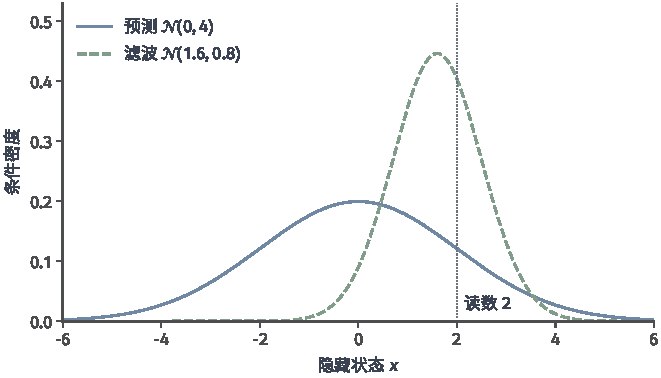
\includegraphics[width=\linewidth]{figures/00-shared/mathematical-preliminaries-lower/02-dynamical-systems-control-decision-and-games/matplotlib/dynamical-kalman-density-update/figure.pdf}
  \caption{独立标量教学例的预测$\mathcal N(0,4)$与后验$\mathcal N(1.6,0.8)$，
 实际读数$y=2$、观测噪声方差$1$。第二个高斯参数是方差；
 本图不是贯穿温度模型的参数设定。}
 \label{fig:dynamical-kalman-density-update}
\end{figure}
\FloatBarrier

若状态更新为$\bm x_{t+1}=\bm f_t(\bm x_t)+\bm w_{t+1}$，
观测为$\bm y_t=\bm h_t(\bm x_t)+\bm v_t$，查询仍是同一个滤波分布，
只是高斯闭合一般失效。扩展Kalman滤波（EKF）在滤波均值附近以
$\bm F_t=D\bm f_t(\bm m_{t\mid t})$传播协方差，
预测均值取$\bm f_t(\bm m_{t\mid t})$；
在预测均值处以$\bm H_{t+1}=D\bm h_{t+1}(\bm m_{t+1\mid t})$
构造创新协方差和增益。它把局部函数替换为一阶线性函数，
所以通常既忽略曲率对均值的影响，也把后验压回单个高斯。

无迹Kalman滤波（UKF）用确定性sigma点近似非线性矩传播。
例如对$d$维均值$\bm m$与协方差$\bm P=\bm L\bm L^\top$，
取$\kappa\geq0$，点为$\bm m$及
$\bm m\pm\sqrt{d+\kappa}\bm L_{\cdot i}$，权重分别为
$\kappa/(d+\kappa)$与$1/[2(d+\kappa)]$。
它们精确匹配原均值与协方差。将点代入$\bm f$，以加权和、加权外积估计
新均值与协方差，再给协方差加上过程噪声$\bm Q$。
本处采用重新生成点的实现：依据加入$\bm Q$后的预测均值和协方差重新构造sigma点，
再把这组点送入$\bm h$，计算预测观测均值、观测协方差及状态观测交叉协方差。
观测协方差还须加上观测噪声$\bm R$，随后按Kalman的创新与增益公式校正。
重新生成点使观测预测也包含本步新增的过程不确定性。
例如标量线性系统$f(x)=h(x)=x$，旧状态方差$p=1$，过程与观测噪声方差
$q=r=1$，上述步骤给出预测方差$2$、创新方差$3$、交叉方差$2$，故增益为$2/3$，
与精确Kalman公式一致；直接复用未包含$q$的原传播点则无法得到这个结果。
这是简单的非负权重构造，实际UKF还可使用带缩放参数的不同权重。
其近似发生在矩积分和高斯投影，不是把非线性模型变成精确线性模型。

两种方法都可能遗漏多峰后验。例如零均值对称先验配上
$y=x^2+v$，一个明显正的读数可能支持正负两个状态区间。
EKF在$x=0$的观测导数为零；对称sigma点也有零状态观测交叉协方差，
单高斯校正不能表达分裂成两峰的证据。
粒子滤波改用加权经验分布$\sum_i\omega_t^{(i)}\delta_{x_t^{(i)}}$：
从已有粒子按转移核抽下一状态，将权重乘当前似然再归一化，
必要时按权重重采样。其近似对象是整个滤波概率测度，
并用有限样本替代核积分；权重集中、高维与重采样损失多样性仍是限制。
高斯混合则保留多个分量，分别传播和校正，再用似然更新分量权重；
分量合并或剪枝会引入另一种近似。

\section{基于完整观测的状态平滑}
滤波只能用到当前时刻为止的读数，适合在线实时估计。但事后做复盘时，我们还掌握了后来的读数，而未来的证据往往能反过来照亮过去——例如事后看到温度后来升得很高，可以推断更早时刻的隐藏状态其实也偏高。
固定终点$T$后，未来读数也能帮助判断旧状态。关键不是再向前预测，
而是把新获得的下一状态分布通过反向条件关系传回去。
在线性高斯条件下，给定$\mathcal Y_t$，
\[
 \begin{bmatrix}\bm x_t\\\bm x_{t+1}\end{bmatrix}
 \sim\mathcal N\left(
 \begin{bmatrix}\bm m_{t\mid t}\\\bm m_{t+1\mid t}\end{bmatrix},
 \begin{bmatrix}
  \bm P_{t\mid t}&\bm P_{t\mid t}\bm A_t^\top\\
  \bm A_t\bm P_{t\mid t}&\bm P_{t+1\mid t}
 \end{bmatrix}\right).
\]
若$\bm P_{t+1\mid t}$可逆，条件高斯公式给出
\begin{align}
 \bm J_t&=\bm P_{t\mid t}\bm A_t^\top\bm P_{t+1\mid t}^{-1},
    \label{eq:dynamical-rts-gain}\\
 \mathbb E[\bm x_t\mid\bm x_{t+1},\mathcal Y_t]
   &=\bm m_{t\mid t}+\bm J_t(\bm x_{t+1}-\bm m_{t+1\mid t}),
    \label{eq:dynamical-rts-one-step-conditional-mean}\\
 \operatorname{Cov}(\bm x_t\mid\bm x_{t+1},\mathcal Y_t)
   &=\bm P_{t\mid t}-\bm J_t\bm P_{t+1\mid t}\bm J_t^\top.
    \label{eq:dynamical-rts-one-step-conditional-covariance}
\end{align}
这里的$\bm J_t$关联相邻状态，不是由当前传感器直接得到的Kalman增益。

\begin{theorem}[有限时域RTS平滑]
 \label{thm:dynamical-rts-smoother}
 在有限时域Kalman条件及每个$\bm P_{t+1\mid t}$可逆条件下，
 从终点$(\bm m_{T\mid T},\bm P_{T\mid T})$向后递推
 \begin{align}
  \bm m_{t\mid T}
   &=\bm m_{t\mid t}+\bm J_t(\bm m_{t+1\mid T}-\bm m_{t+1\mid t}),
       \label{eq:dynamical-rts-smoothed-mean}\\
  \bm P_{t\mid T}
   &=\bm P_{t\mid t}
         +\bm J_t(\bm P_{t+1\mid T}-\bm P_{t+1\mid t})\bm J_t^\top,
       \label{eq:dynamical-rts-smoothed-covariance}
 \end{align}
 精确给出$\bm x_t\mid\mathcal Y_T$的高斯均值与协方差。
\end{theorem}
\begin{proof}
 给定$\bm x_{t+1}$后，未来状态和观测与更早状态条件独立，因此
 $P(\mathrm d\bm x_t\mid\bm x_{t+1},\mathcal Y_T)
   =P(\mathrm d\bm x_t\mid\bm x_{t+1},\mathcal Y_t)$。
 全概率公式给出后向因子化
 \begin{equation}
  P(\mathrm d\bm x_t\mid\mathcal Y_T)
   =\int P(\mathrm d\bm x_t\mid\bm x_{t+1},\mathcal Y_t)
                   P(\mathrm d\bm x_{t+1}\mid\mathcal Y_T).
  \label{eq:dynamical-rts-backward-factorization}
 \end{equation}
 将一步条件均值对$\bm x_{t+1}\mid\mathcal Y_T$取期望，
 塔式性质得到平滑均值公式。全协方差公式分成两项：条件内协方差为
 $\bm P_{t\mid t}-\bm J_t\bm P_{t+1\mid t}\bm J_t^\top$，
 条件均值的协方差为$\bm J_t\bm P_{t+1\mid T}\bm J_t^\top$；
 相加即得平滑协方差。一步条件核的均值为仿射函数、协方差不依赖下一状态，
 与高斯下一状态混合仍为高斯。从$T$向后归纳，完成全部时刻的结论。
\end{proof}

前向保存每步滤波与预测的均值、协方差，后向依次计算$\bm J_t$及上述两式，
就是Rauch--Tung--Striebel（RTS）平滑算法\scite{math-rauch1965smoothing}
未来观测影响过去的条件分布，不改变已经发生的物理状态。

\begin{example}[未来观测降低过去状态的不确定性]
 \label{ex:dynamical-scalar-rts-update}
 用独立随机游走例$x_1=x_0+w_1$、$y_1=x_1+v_1$，
 取$m_{0\mid0}=0,P_{0\mid0}=1,Q_1=1,R_1=2/3$，
 初值及两类噪声相互独立，且均为零均值高斯。
 观察$y_1=2$后，$m_{1\mid0}=0,P_{1\mid0}=2$，
 $K_1=3/4,m_{1\mid1}=3/2,P_{1\mid1}=1/2$。
 于是$J_0=1/2$，$m_{0\mid1}=3/4$，
 $P_{0\mid1}=1+\frac14(\frac12-2)=5/8$。
 在时刻$0$尚不能使用这个结果；此时只有均值$0$、方差$1$的初始先验。

 这里每一步的算术都可以顺次核对。先由
 $P_{1\mid0}=P_{0\mid0}+Q_1=1+1=2$得到预测方差，再看增益
 $K_1=P_{1\mid0}/(P_{1\mid0}+R_1)=2/(2+2/3)=3/4$。读数$y_1=2$比预测均值
 $m_{1\mid0}=0$高出\(2\)，于是滤波均值取预测与读数的加权位置
 $m_{1\mid1}=0+\frac34\times2=3/2$——更接近读数，因为观测噪声方差
 \(2/3\)小于预测方差\(2\)。滤波方差降为
 $P_{1\mid1}=2\times(2/3)/(2+2/3)=1/2$。
 后向一步用
 $J_0=P_{0\mid0}/P_{1\mid0}=1/2$：下一状态比预测高出\(3/2\)，
 按这个比例把一半回传到时刻\(0\)，得$m_{0\mid1}=\frac34$；
 平滑方差$P_{0\mid1}=5/8<1=P_{0\mid0}$，说明关于$x_0$的不确定性
 确实被后来的读数缩小了。

 这组数字应按目标状态的时刻分成两组比较。固定目标$x_1$时，
 尚未取得$y_1$的预测均值、方差为$(0,2)$；加入$y_1$后，
 滤波结果为$(3/2,1/2)$。固定目标$x_0$时，无观测的先验为$(0,1)$；
 取得后续读数$y_1$后，平滑结果变为$(3/4,5/8)$。
 每组都保持目标状态不变，只增加所用的观测信息。

 在时刻$0$，$y_1$尚未获得，因此只能使用$x_0$的先验；
 到时刻$1$，既可以用$y_1$估计当前的$x_1$，也可以回溯估计过去的$x_0$，
 两个查询的目标时刻不同。在这个$T=1$的窗口中，$x_1$的平滑已经等于滤波；
 若要比较同一$x_1$在滤波后再吸收更晚读数的变化，还须增加$y_2$等后续观测。
\end{example}

\begin{figure*}[!htb]
  \centering
  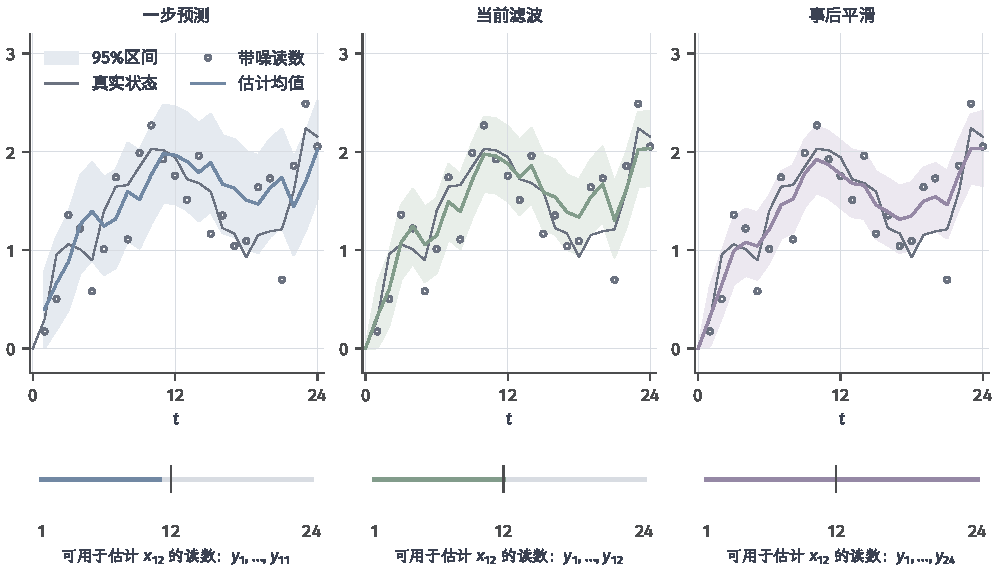
\includegraphics[width=\linewidth]{figures/00-shared/mathematical-preliminaries-lower/02-dynamical-systems-control-decision-and-games/matplotlib/action-state-temperature-inference/figure.pdf}
  \caption{与图~\ref{fig:action-state-temperature-layers}完全相同的温度轨迹及读数。
 三栏分别画一步预测、滤波与固定终点$T=24$的平滑均值和逐时刻$95\%$高斯区间，
 灰线为实际状态，圆点为读数；区间不是整条路径同时覆盖的置信带。
 下方以$t=12$为例标出可用观测范围。已知$x_0=0$，给定$u_t=0.4$，
 过程、观测方差仍为$0.04,0.09$。平滑的信息优势不是额外的在线能力。}
 \label{fig:action-state-temperature-inference}
\end{figure*}

沿用上述有限时域线性高斯条件，有$\bm P_{t\mid T}\preceq\bm P_{t\mid t}$，
即滤波协方差减去平滑协方差是半正定矩阵。这也可从RTS协方差公式向后归纳：
终点两者相等，下一步的平滑协方差不超过其预测协方差，夹乘$\bm J_t$后仍为半正定差。
但某一条实现上的均值误差不必
每个时刻都更小。条件均方误差的保证与某一次噪声实现上的误差是不同对象。
若预测协方差奇异，须在其仿射支持上条件化，广义逆只是计算工具，
还要检查条件状态是否属于支持，不能只替换逆号。
非线性近似平滑可沿相同后向关系用局部线性化或sigma点估计相邻状态的交叉矩；
粒子平滑则近似反向核或路径权重。无论采用哪种表示，使用$\mathcal Y_T$
这一信息条件都不改变。

\section{基于完整观测的联合轨迹推断}
各时刻边缘分布回答“那一刻可能在哪里”，整条路径后验还要回答“这些状态如何
一起出现”。在共同观测密度条件下，
\begin{equation}
 P(\mathrm d\bm x_{0:T}\mid\bm y_{1:T})
   =\frac1{Z(\bm y_{1:T})}\,
      \pi_0(\mathrm d\bm x_0)
      \prod_{t=0}^{T-1}K_t(\bm x_t,\mathrm d\bm x_{t+1})
      \prod_{t=1}^Tg_t(\bm y_t\mid\bm x_t),
 \label{eq:action-state-trajectory-posterior}
\end{equation}
其中证据$Z$是分子对路径的积分，要求$0<Z<\infty$。
乘积记号按转移核的迭代积分理解，不预设状态本身有Lebesgue密度。
每个平滑边缘由这一个联合后验积分而来；反过来，只给全部边缘并不能恢复跨时刻关联。

若损失为$\sum_t\|\bm x_t-\bm a_t\|^2$，联合条件均值的各分量就是
$\bm m_{t\mid T}$，因此逐时刻平滑均值同时组成最小化该可加平方损失的路径输出。
在线性高斯模型中，把所有状态堆叠为$\bm X$后，后验仍为联合高斯。
协方差$\bm\Sigma\succ\bm0$时，其密度正比于
$\exp[-(\bm X-\bm m)^\top\bm\Sigma^{-1}(\bm X-\bm m)/2]$，
故联合众数为$\bm m$，也与各时刻的边缘众数一致。
这是一项高斯结构结论，不是所有后验的性质。

若$\bm\Sigma$奇异，后验集中在仿射支持
$\bm m+\operatorname{range}(\bm\Sigma)$，没有全维Lebesgue密度。
记$r=\operatorname{rank}(\bm\Sigma)$。若$r=0$，后验就是点质量$\delta_{\bm m}$，
直接取$\bm m$为输出。若$r>0$，写$\bm\Sigma=\bm U_r\bm\Lambda_r\bm U_r^\top$，
在支持坐标$\bm z=\bm U_r^\top(\bm X-\bm m)$中才有非退化高斯密度；
其唯一众数为$\bm z=\bm0$，对应$\bm m$。
条件高斯使用广义逆时也须要求所给证据位于其支持内；
支持外的条件值属于零概率事件，公式不能赋予一个未经指定的后验意义。

非高斯下可直接看出区别。设两个时刻的联合后验为
\[
 \begin{aligned}
  P(x_0=0,x_1=0)&=0.40,\\
  P(x_0=0,x_1=1)&=0.25,\\
  P(x_0=1,x_1=1)&=0.35.
 \end{aligned}
\]
其他组合概率为零。它可由初始概率$(0.65,0.35)$和转移
$P_{00}=8/13,P_{01}=5/13,P_{11}=1$生成，再配无信息观测。
时刻$0$的边缘众数为$0$，时刻$1$的边缘众数为$1$；
拼接得到$(0,1)$，联合概率只有$0.25$，低于联合最优路径$(0,0)$的$0.40$。
逐点多数意见没有保留跨时刻相容性的全部权重。

有限状态的联合MAP可沿链做最大乘积或Viterbi递推，
而边缘查询沿链求和；其局部函数计算回见图论。
连续非高斯模型可能用路径优化求一个MAP，也可能用粒子或Monte Carlo方法
近似整个后验；前者不是后者的替代品。
例如由$\bm x_T\mid\mathcal Y_T$抽样，再逐步按反向条件核抽
$\bm x_t\mid\bm x_{t+1},\mathcal Y_t$，得到的是有关联的后验路径；
独立从每个平滑边缘抽样会丢掉这些关联。
相关工具可参考\BookPartRef{part:graphs}{卷1《数学准备：计算、分析与几何》的“图”部分}。

本节的精确结论都在有限时域成立。稳态增益、极限协方差及估计误差的长期稳定性，
仍需可检测性、噪声作用方向等系统条件；这些问题交由
\BookChapterRef{chap:control-theory}{第~\ref{chap:control-theory}章}处理。在那里输入才由反馈主动选择，
本章一直把$\bm u_t$当作已给定量。

\section{本章小结}
\label{sec:state-space-estimation-summary}

同一温度模型中，演化规律、真实轨迹与传感器读数承担不同职责：过程噪声使轨迹成为随机对象，观测噪声产生用于推断的记录。
推断不是再生成一条任意轨迹，而是在给定生成模型中按读数重新分配状态的概率。

预测、滤波、平滑和联合轨迹推断按可用观测范围与查询对象区分。
预测只用过去读数，滤波加入当前读数，平滑使用整段记录；它们输出的是条件分布或其摘要，而联合轨迹推断还要保留跨时刻的相关性，逐时刻的边缘众数拼接未必是联合最可能的路径。
线性高斯模型下，Kalman滤波与RTS平滑把这些条件分布精确写成均值与协方差的递推；非线性或非高斯模型需要另选近似表示，但条件信息的定义不变。

本章的精确结论都在有限时域成立，输入被当作已给定量。稳态增益、误差的长期稳定以及怎样选择输入，需要可检测性等系统条件，留给\BookChapterRef{chap:control-theory}{“控制”部分的相应章节}。
